\documentclass[11pt,a4paper]{article}
\usepackage{amsmath, tabularx, geometry, graphicx, xcolor, multirow}

\usepackage{tikz}
\usetikzlibrary{positioning}
\newdimen\nodeDist
\nodeDist=35mm

\geometry{a4paper, left=20mm, top=20mm}
\graphicspath{{./imgs/}}
\renewcommand\tabularxcolumn[1]{m{#1}}

\title{Aprendizagem 2021/22 Homework I - Group 66}
\author{João Cardoso, 99251. José João Ferreira, 99259}

\begin{document}

\color{darkgray}
\hspace{-8.25mm}
\begin{tabularx}{1.09\textwidth} {>{\raggedright\arraybackslash}X >{\centering\arraybackslash}X >{\raggedleft\arraybackslash}X}
  \includegraphics[scale=0.2]{tecnico.pdf} &
  \textbf{Aprendizagem 2022/23} \par \textbf{Homework I - Group 66} &
  João Cardoso, 99251 \par José João Ferreira, 99259
\end{tabularx}
\color{black}

\begin{center}
\textbf{I. Pen-and-paper}
\end{center}

% PROBLEM 1
\begin{flushleft}
\textbf{1)}
\small
\begin{tabular}{llcc}
                                                  &                        & \multicolumn{2}{c}{Real}                        \\ \cline{3-4} 
                                                  & \multicolumn{1}{l|}{}  & \multicolumn{1}{c|}{P} & \multicolumn{1}{c|}{N} \\ \cline{2-4} 
  \multicolumn{1}{c|}{\multirow{2}{*}{Predicted}} & \multicolumn{1}{c|}{P} & \multicolumn{1}{c|}{8} & \multicolumn{1}{c|}{4} \\ \cline{2-4} 
  \multicolumn{1}{c|}{}                           & \multicolumn{1}{c|}{N} & \multicolumn{1}{c|}{3} & \multicolumn{1}{c|}{5} \\ \cline{2-4} 
\end{tabular}

\normalsize
\end{flushleft}

% PROBLEM 2
\begin{flushleft}
\textbf{2)}
\small
\hspace{-8.25mm}
\vspace{4mm}
\begin{tabularx}{1.09\textwidth}{XXX}
  
  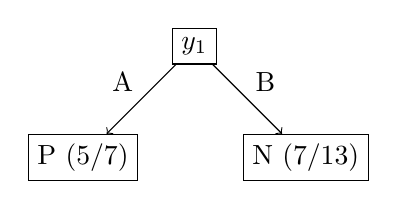
\begin{tikzpicture}[node/.style={draw,rectangle}, ->]
    \node [node] (node_1) {$y_1$};
    \path (node_1) ++ (-135:2) node [node] (node_2) {P (5/7)};
    \path (node_1) ++ (-45:2) node [node] (node_3) {N (7/13)};
    \draw (node_1) -- (node_2) node [left,pos=0.25] {A\hspace{2mm} }(node_1);
    \draw (node_1) -- (node_3) node [right,pos=0.25] {\hspace{2mm}B}(node_1);
  \end{tikzpicture} &

  \begin{tabular}{llcc}
    &                        & \multicolumn{2}{c}{Real}                        \\ \cline{3-4} 
    & \multicolumn{1}{l|}{}  & \multicolumn{1}{c|}{P} & \multicolumn{1}{c|}{N} \\ \cline{2-4} 
  \multicolumn{1}{c|}{\multirow{2}{*}{Predicted}} & \multicolumn{1}{c|}{P} & \multicolumn{1}{c|}{5} & \multicolumn{1}{c|}{2} \\ \cline{2-4} 
  \multicolumn{1}{c|}{}                           & \multicolumn{1}{c|}{N} & \multicolumn{1}{c|}{5} & \multicolumn{1}{c|}{7} \\ \cline{2-4} 
  \end{tabular} &
  \normalsize
  $ Precision = \frac{TP}{TP + FP} = \frac{5}{5 + 2} = \frac{5}{7} $ \par
  $ Recall = \frac{TP}{TP + FN} = \frac{5}{5 + 5} = \frac{1}{2} $
\end{tabularx}
\vspace{0mm}
\normalsize
$ F_{\beta = 1} = \frac{1}{\frac{1}{2Precision} + \frac{1}{2Recall}} = \frac{1}{\frac{7}{10} + \frac{2}{2}} = \frac{1}{\frac{17}{10}} = \frac{10}{17} \approx 0.588235 $ \par
\end{flushleft}
\vfill

% PROBLEM 3
\begin{flushleft}
\textbf{3)}
Some values of $y_2$, given $y_1 = A$, might be missing or corrupted. Another reason could be a very low information gain about $y_{out}$ of the variable $y_2$, given $y_1 = A$.
\end{flushleft}
\vfill

% PROBLEM 4
\begin{flushleft}
\textbf{4)}
\small
\hspace{-8.25mm}
\begin{tabularx}{1.09\textwidth}{>{\hsize=.25\hsize}X X}
  \vspace{-20mm}
  \begin{tabular}{ccc}
  $y_1$ & $y_2$                 & $y_{out}$ \\ \hline
  A     &                       & P         \\ \hline
  A     &                       & P         \\ \hline
  A     &                       & P         \\ \hline
  A     &                       & P         \\ \hline
  A     &                       & P         \\ \hline
  A     &                       & N         \\ \hline
  A     &                       & N         \\ \hline
  B     & \textgreater 2        & P         \\ \hline
  B     & \textgreater 2        & P         \\ \hline
  B     & \textgreater 2        & P         \\ \hline
  B     & \textgreater 2        & N         \\ \hline
  B     & \textgreater 2        & N         \\ \hline
  B     & \textgreater 2        & N         \\ \hline
  B     & \textgreater 2        & N         \\ \hline
  B     & \textgreater 2        & N         \\ \hline
  B     & $\leq$2               & P         \\ \hline
  B     & $\leq$2               & P         \\ \hline
  B     & $\leq$2               & P         \\ \hline
  B     & $\leq$2               & N         \\ \hline
  B     & $\leq$2               & N         \\
  \end{tabular} &
  
  \normalsize\vspace{10mm}
  $ E(y) = -\sum_{v \in y} P(v)\log_2(P(v)) $
  \newline\newline
  $ E(y_{out}) = -\frac{11}{20}\log_2(\frac{11}{20}) -\frac{9}{20}\log_2(\frac{9}{20}) $ \par\vspace{1mm}
  \hspace{12.25mm} $ \approx 0.992774 $
  \newline\newline
  $ E(y_{out}|y_1) = \frac{7}{20}[-\frac{5}{7}\log_2(\frac{5}{7}) -\frac{2}{7}\log_2(\frac{2}{7})] + \frac{13}{20}[-\frac{7}{13}\log_2(\frac{7}{13}) -\frac{6}{13}\log_2(\frac{6}{13})] $ \par\vspace{1mm}
  \hspace{16.75mm} $ \approx 0.949315 $ 
  \newline\newline
  $ IG(y_{out}|y_1) = E(y_{out}) - E(y_{out}|y_1) $ \par\vspace{1mm}
  \hspace{18.75mm} $ = 0.992774 - 0.949315 $ \par\vspace{1mm}
  \hspace{18.75mm} $ = 0.043459 $
  
\end{tabularx}
\end{flushleft}

\begin{center}
\textbf{II. Programming}
\end{center}

% PROBLEM 1
\begin{flushleft}
\textbf{1)}
\end{flushleft}
  
% PROBLEM 2
\begin{flushleft}
\textbf{2)}
\end{flushleft}

\begin{center}
\textbf{III. Appendix}
\end{center}

{\fontfamily{cmtt}\selectfont
This text uses a different font typeface.
Paste your programming code here using Consolas 9pt or 10pt.
Use highlighted or colored text to facilitate the analysis by your faculty hosts.
}

\end{document}